\documentclass[landscape]{sciposter}
%\documentclass[landscape,draft]{sciposter}
\usepackage[]{graphicx}
\usepackage{amsmath,amsfonts,amssymb}
\usepackage{units}
\usepackage{authoraftertitle}
\usepackage[utf8]{inputenc}
\usepackage[T1]{fontenc}
\usepackage{charter}
\usepackage[expert]{mathdesign}
\usepackage{siunitx}
%\usepackage{fancyhdr}
%\usepackage{etoolbox}
%\renewcommand{\familydefault}{\rmdefault}

\usepackage{multicol}
\usepackage{url}

% Set the lengths of the pictures
\newlength{\customfigwidth}
\setlength{\customfigwidth}{16cm}

\newlength{\customfigheight}
\setlength{\customfigheight}{12cm}

\setlength{\belowdisplayskip}{10pt} \setlength{\belowdisplayshortskip}{10pt}
\setlength{\abovedisplayskip}{10pt} \setlength{\abovedisplayshortskip}{10pt}
\setlength{\columnseprule}{4pt}
\setlength{\multicolsep}{6.0pt plus 2.0pt minus 1.5pt}% 50% of original values
\setlength\columnsep{40pt}% 50% of original values

\newcommand{\eqnote}[1]{{\scriptsize#1}}


\usepackage[font={large,it}]{caption}
\usepackage[protrusion=true,expansion=true]{microtype}

% Convenience functions
\newcommand{\pfrac}[2]
        {\frac{\partial #1}{\partial #2}}       % partial 1 /partial 2 
\newcommand{\ket}[1]
        {\left | \, #1 \right \rangle}          % bra-ket notation
\newcommand{\abs}[1]{
        \left\vert #1 \right\vert}		% vert bars for averages
\newcommand{\norm}[1]
        {\left\Vert #1 \right\Vert}             % taller vert bars for the norm
\newcommand{\evalat}[1]
        {\left. #1 \right \vert}        % ex. evaluating the int. at its limits
\newcommand{\set}[1]
        {\left\{ #1 \right\}}           % squigle brackets for sets
\newcommand{\avg}[1]
        {\left< #1 \right>}		% angle brackets for averages < >
\newcommand{\paren}[1]
        {\left( #1 \right)}		% grows parentheses () 
\newcommand{\brackets}[1]
        {\left[ #1 \right]}		% grows square brackets []
\newcommand{\braces}[1]
        {\left \{ #1 \right \}}         % grows curly brackets {}
\newcommand{\piecewisebrace}[1]
        {\left \{ #1 \right .}          % piecewisebrace

% Shorthand with proper spacing
\newcommand{\viz}{viz.\ }
\newcommand{\ie}{i.e.\ }
\newcommand{\eg}{e.g.\ }
\newcommand{\cf}{c.f.\ }

% Chemical formula
\newcommand{\chem}[1]{\ensuremath{\mathrm{#1}}} 

% New math operators
\DeclareMathOperator*{\minor}{minor\,}
\DeclareMathOperator*{\sgn}{\mathbf{sgn}\, }
\DeclareMathOperator*{\rootof}{RootOf\,}

% Vector notation
\newcommand{\mathvect}[1]{\boldsymbol{#1}}
\newcommand{\vect}[1]{\mathbf{#1}}

% Differential used at the end of an integral
\newcommand*\diff{\mathop{}\!\mathrm{d}}
\newcommand{\integral}[2]{\int #1\diff#2}


% Equation placeholders
\newcommand{\SPHYvals}{%
  Y_{\ell m}^{*} ( \hat{\vect{r}}_i ) 
  Y_{\ell m}     ( \hat{\vect{r}} ) 
}

\newcommand{\SPHsumterms}{%
    \sum_{\ell=0}^\infty \sum_{m=-\ell}^{\ell} %
}

\newcommand{\SPHsum}[1]{%
  \SPHsumterms
  #1
  \SPHYvals
}

\newcommand{\normdiff}[1]{%
  \norm{ \vect{#1} - \vect{#1}_i}
}

\newcommand{\ViralInteractionPot}{\Phi_{12}}
\newcommand{\transpose}[1]{^{\intercal}}

\newcommand{\sphericalBesselIN}{ i }
\newcommand{\sphericalBesselKN}{ k }
\newcommand{\knownPHI}{\Psi}
\newcommand{\macroPHI}{\Phi}

\newcommand{\pka}{\text{pKa}}
\newcommand{\pH}{\text{pH}}
\newcommand{\LMAX}{\ell_{\text{MAX}}}

\newcommand{\effChargeLocations}{\vect{r}_1, \vect{r}_2, \ldots, \vect{r}_N}
\newcommand{\fittingACCeffective}{\chi}
\newcommand{\debyehukel}{Debye-H\"{u}ckel }

%\definecolor{BoxCol}{rgb}{.93531, .93531, .93531}
%\definecolor{palered}{RGB}{255,182,182}


\newcommand{\titlefont}[1]{%
  {%
  \usefont{T1}{bch}{b}{n}%
    \selectfont%
    #1%
  }%
  \normalfont%
}

\newcommand{\at}{\makeatletter\titlefont{@}\makeatother}


\author{Travis Hoppe, Robert Best}
\email{hoppeta@mail.nih.gov}
\institute{National Institutes of Health, National Institute of Diabetes and Digestive and Kidney Diseases}
\conference{\titlefont{\large Biophysical Society Meeting 2016, Los Angeles CA}}

\renewcommand{\sectionsize}{%
  \usefont{T1}{bch}{b}{n}%
  \scshape%
  \bfseries%
  \large
  \selectfont%
}
 
\begin{document}

% Custom footer
\renewcommand{\footlogo}{%
  \resizebox{2\logowidth}{!}{%
    
\includegraphics[height = 1cm]{logos/NIDDK_logo.pdf}%
    \hspace{1em}
    
\includegraphics[height = 1cm]{logos/dhhs_logo.pdf}%
    \hspace{1em}
    
\includegraphics[height = 1cm]{logos/NIH_Logo.pdf}
  }
}

% Custom title
%\maketitle
\resizebox{\textwidth}{!}{
  \begin{tabular}{ p{.6\textwidth} r }
    \titlefont{\Huge  Enhancing the Coevolutionary Signal }  &
    \titlefont{\Large \MyAuthor} \\
    %& 
    \titlefont{\Large via machine learning}&
    %\includegraphics[height = 1cm]{mail.png}
    \texttt{hoppeta}{\bfseries \at}\texttt{mail.nih.gov}
    %&
  \end{tabular}
}
\vspace{1cm}


\begin{multicols}{3}

\section*{Abstract}
Analysis of coevolutionary relationships between residue pairs in the sequences of folded proteins can yield information on which residues interact in the folded state, and hence produce a contact map based only on sequence information. 
The distribution of contacts in folded proteins is far from random, as evident from looking at any contact map. 
Therefore, it should be possible to use information from neighboring contacts in order to strengthen the predictive power of coevolutionary analysis. 
Here, we show that application of a machine-learning algorithm to contact maps from analysis of evolutionary couplings significantly improves the precision of the derived contact map with a sacrifice in sensitivity, so that many more contacts can be predicted with confidence. 

%Since this does not immediately guarantee that this improvement would carry over to improvements in structure prediction, we have also investigated the effect of the contact map refinements on the quality of structures predicted using a simple coarse-grained folding algorithm.
% We again find that our contact map refinement yields structures which are closer to the experimentally determined native state, over a set of diverse protein folds.
\vfill
\columnbreak

\section*{Methods}

Download, parse, and clean PDB.
Build FASTA and reference contact map.
Align each FASTA using HHBLITS*.
Score alignments with GREMLIN.
Build contact maps from GREMLIN.
(optional) Optimize contact map score with RF.
Fold coarse-grained protein from contact map.

Scoring: For a given protein and alignment GREMLIN gives $(N,N,21,21)$ tensor.

Reduce GREMLIN's tensor output: 
$S_{N,N,21,21} \rightarrow S_{N,N,20,20} \rightarrow  G_{N,N} \rightarrow G^{\text{APC}}_{N,N} = g$ 
Drop information about gaps.
Compute the Frobenius norm over each position. Subtract average product correlation, structural vs. shared ancestry $APC(a,b) = MI(a,\overline{x}) MI(b,\overline{x}) / \overline{\text{MI}}$

Protein dataset taken from PSICOV\cite{jones2012psicov}.

\vfill
\columnbreak

\section*{Coevolutionary Analysis: GREMLIN\cite{kamisetty2013assessing}}


Optimize the pseudolikelihood of $v,w$

$$ P(v,w | D) = \sum_{n=1}^N \sum_{i=1}^L \log P (x_i^n | x_{i'}^n, v, w)$$

$$ P (x_i^n | x_{i'}^n, v, w) = \frac{1}{Z_i} \exp \left ( v_i(x_i^n) + \sum_{j=1,j \neq i}^L w_{ij}(x_i^n,x_j^n) \right )$$
Models conditional distribution of the original joint distribution instead of the joint distribution itself. 
Can add regularization to prevent overfitting and prior knowledge. 
$v_i$ encodes individual propensity of each amino acid at position $i$ $w_{ij}$ statistical coupling of amino acid propensities between positions $i,j$

\end{multicols}

\begin{multicols}{3}
\section*{Hypothesis}

RANDOM FOREST (RF) SCORE MODEL
Machine learn local pixel maps for contact/non-contact.
Normalize data: subtract mean, scale to unit variance.
Train with extremely random forests*, variant with dropout.
(e)RF's were more robust than traditional shallow learning like SVM.
\vfill \columnbreak

\section*{Improved Contact Maps}

\begin{figure}
    \center 
    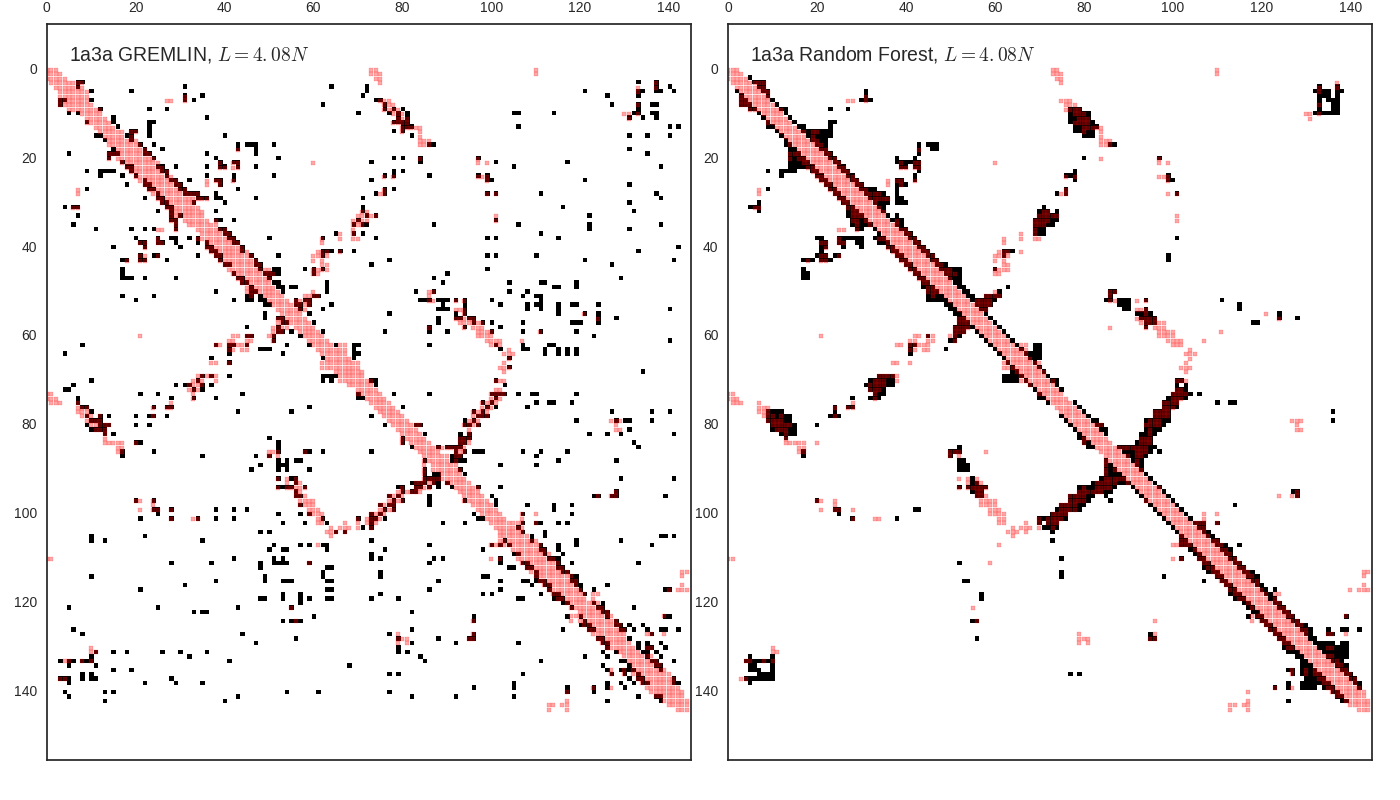
\includegraphics[height=1.25\customfigheight]{figures/1a3a_cmp.png}%
\caption{$\SI{8}{\angstrom}$  $C_\alpha$ contact map of protein 1a31 (IIA Mannitol from E. Coli) in red, original GREMLIN scoring method on the left and improved RF-GREMLIN method on the right. Using the traditional scoring method, false positives appear uniformly randomly across the contact pairs, while the RF method is more precise and accurate by concentrating local information. }
\end{figure}

\vfill \columnbreak

\section*{ROC Curve}
\begin{figure}
    \center 
    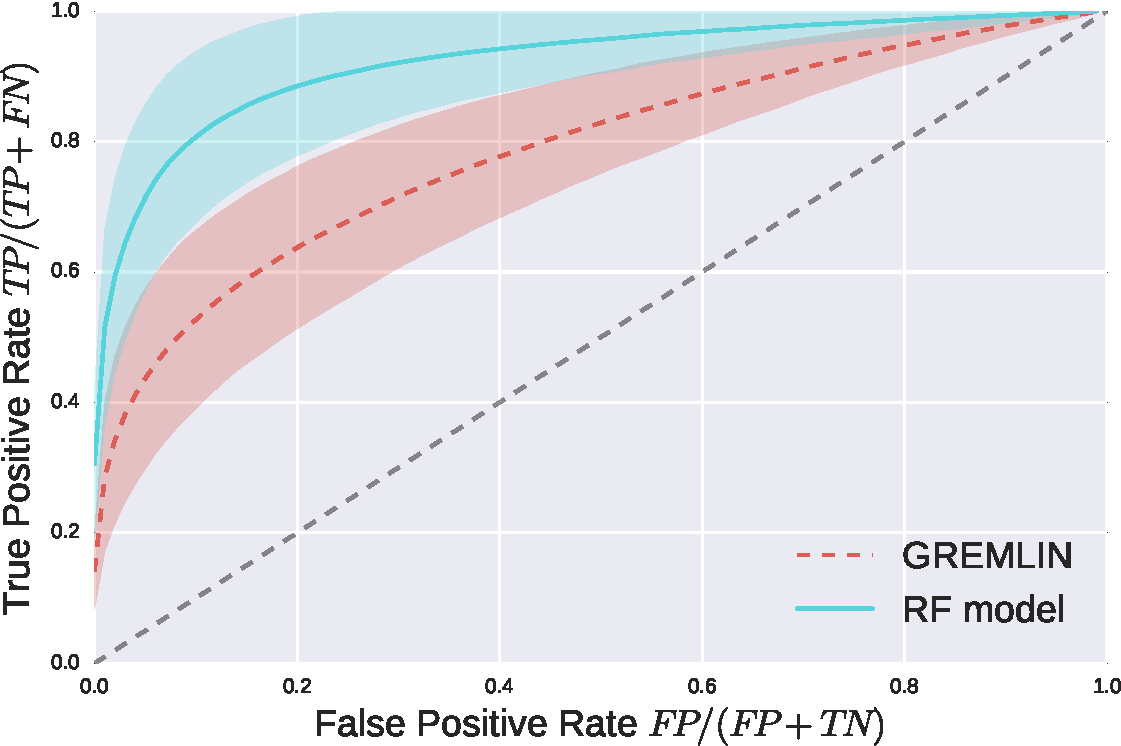
\includegraphics[height=\customfigheight]{figures/GREMLIN_RF_ROC-crop.pdf}%
    \hfill%
    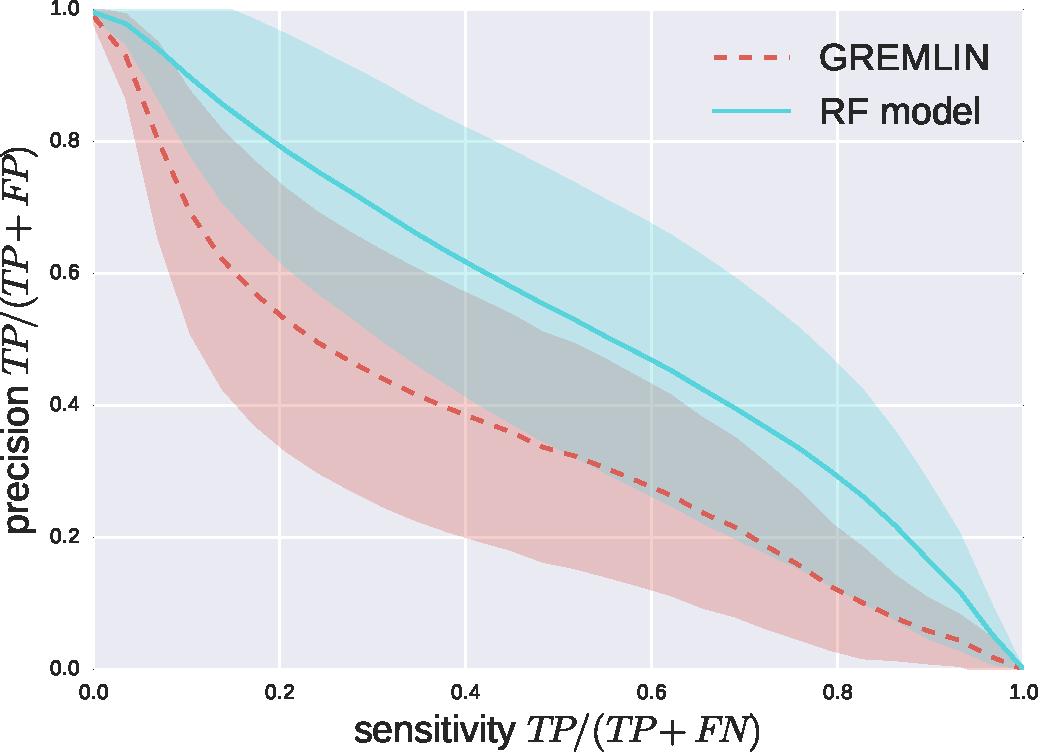
\includegraphics[height=\customfigheight]{figures/GREMLIN_RF_Acc_Pre-crop.pdf}%
\caption{%
Left: Receiver operating curve, Right: Sensitivity vs. Precision.
For any given sensitivity, RF-GREMLIN outperforms the traditional GREMLIN by choosing more correct contacts.
}

\end{figure}

\end{multicols}

\begin{multicols}{3}

\section*{Q-values plots}
\begin{figure}
    \center 
    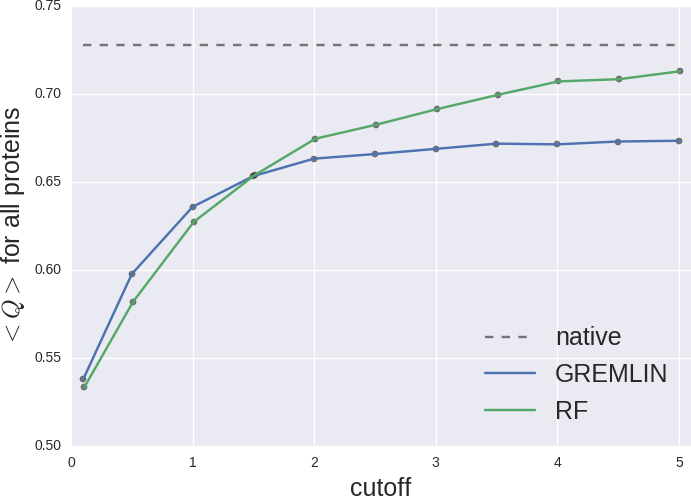
\includegraphics[height=1.5\customfigheight]{figures/folding/Q_avg.png}

\caption{
Folding simulations
$C_\alpha$ coarse-grained MD simulation
Unbiased estimate of contact map $\rightarrow$ fold.
No prior knowledge (ROSETTA fragments, SS predictions., etc...).
Potential = Backbone + smoothed well with range ~ $\SI{8}{\angstrom}$.
}
\end{figure}

\vfill \columnbreak

\section*{Contact improvement is localized}

\begin{figure}
    \center 
    \hfill%
    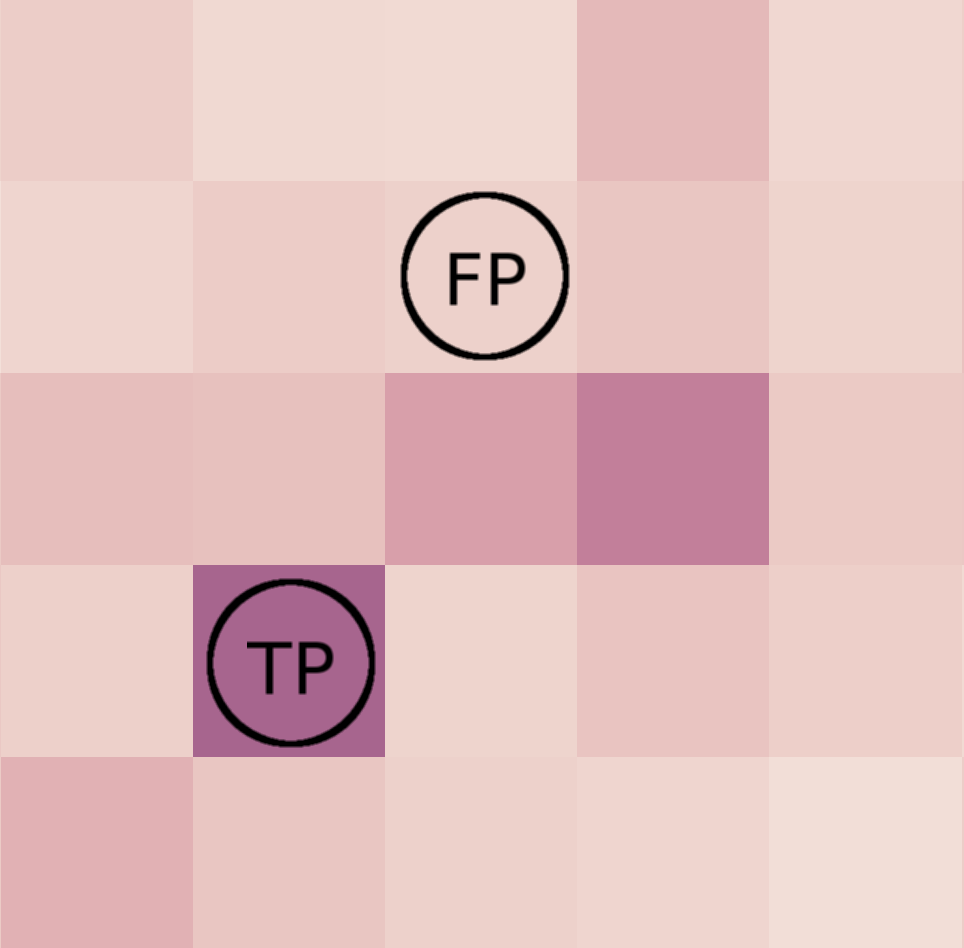
\includegraphics[height=\customfigheight]{figures/local_structure_distance.png}%   
    \hfill%
    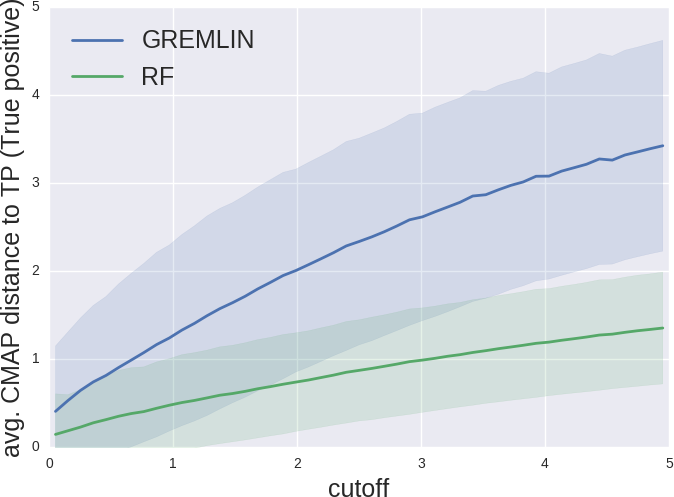
\includegraphics[height=\customfigheight]{figures/FP_distance.png}%
    \hfill%
    \hspace{0em}

\caption{%
Both methods give false positive results, but the predictions by RF-GREMLIN were correlated to the true positives. We measured the average city-block (L1-norm) distance from each false positive to the nearest true positive averaged all protein datasets. Left: diagrammatic illustration of a false positive (FP) to true positive (TP) distance of three. Right: Averaged L1 distance for all FP to TP across the dataset.
}
\end{figure}

\vfill \columnbreak

\section*{Feature selection}

\begin{figure}
    \center 
    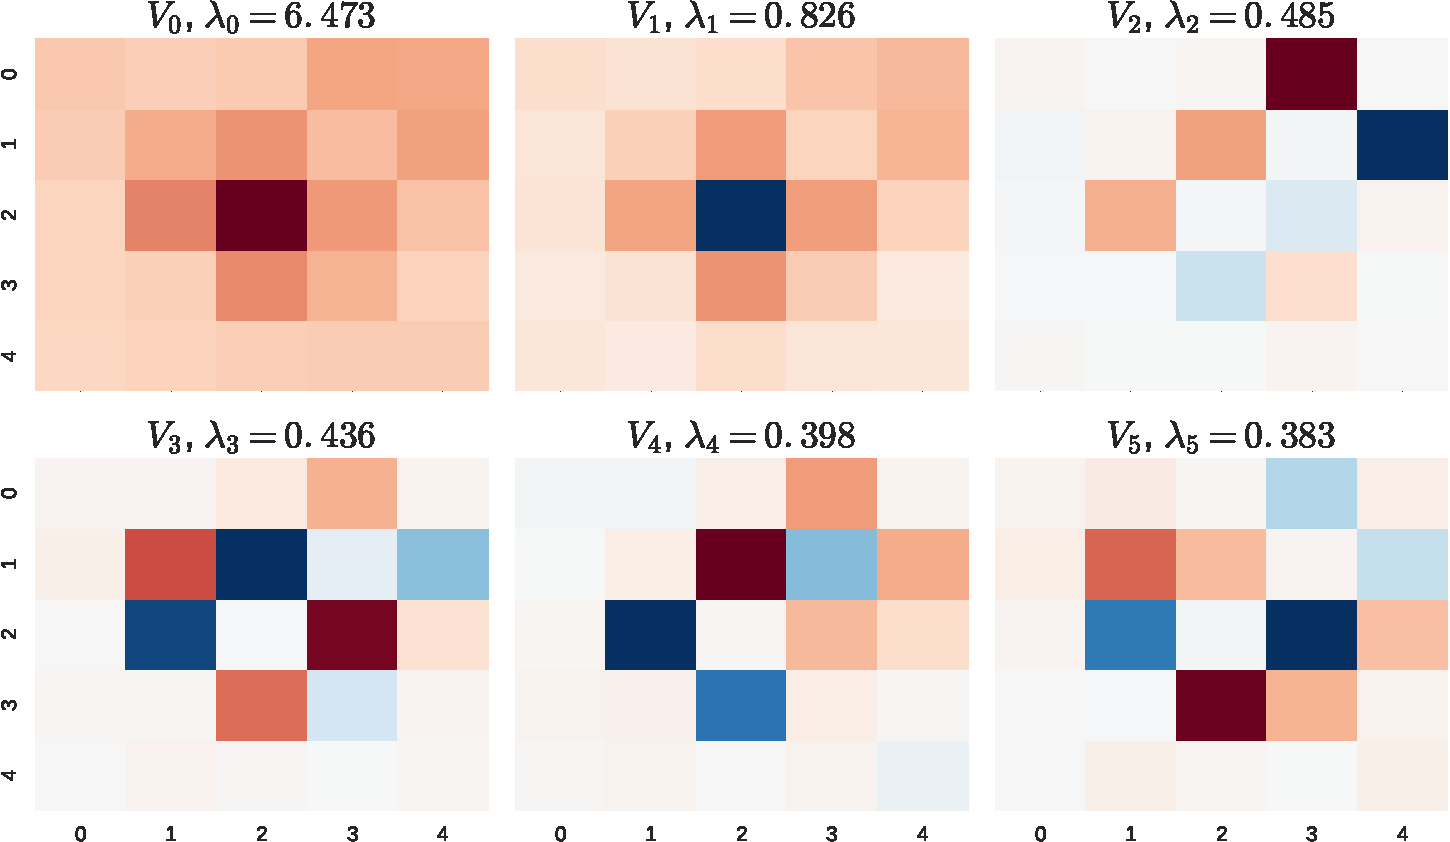
\includegraphics[width=1.5\customfigwidth]{figures/avg_features-crop.pdf}%
\caption{
Singular value decomposition of RF terminal leaf nodes to illustrate feature selection. The dominant features ($V_1, V_2$) are roughly described by a Gaussian kernel and the difference between the center and the outlying values.
}
\end{figure}


\renewcommand{\refname}{} 
\bibliographystyle{unsrt}
%\bibliographystyle{plain}  % enter bibligraphy as usual, with or without using
\small                     
\bibliography{bib/CMAP.bib} 

%\renewcommand{\refname}{xxx} 
%\begin{sectionbox}{}  
% changes section heading over bibliography

%\bibliography{../bib/AnisoChargeFits.bib}
%\end{sectionbox}

\end{multicols}

 
\end{document}
